\section{Data and Methods}
\label{sec:data_methods}

\subsection{Hydrodynamic model}
\label{sec:methods_model}

Circulation was simulated with D-Flow Flexible Mesh (D-Flow FM, kernel
1.2.184) from the Delft3D FM Suite 2026.01, an unstructured finite-volume
solver for the three-dimensional shallow-water equations \citep{Kernkamp2011}.
The mesh of 25{,}212 faces covers the lagoon together with an offshore
extension reaching the western Sicilian channel, spanning 11.96--12.56$^\circ$E
and 37.70--38.06$^\circ$N, and grades from about 880~m offshore to about 60~m
in the lagoon and along the shorelines, so that about six cells span the 400~m
northern inlet. The vertical carries 10 sigma layers of uniform thickness,
about 0.095~m at the mean depth of 0.95~m, which resolves the wind-driven
surface drift over the near-bed return flow reported by \citet{DeMarchis2012}
and spreads the 0.40~m canopy of Section~\ref{sec:methods_roughness} over the
lowest four layers and part of the fifth.

Turbulence closure used the $k$--$\varepsilon$ model, and density followed the
UNESCO equation of state with salinity and temperature as active constituents,
so that the summer hypersaline gradient contributes baroclinically. Bed
roughness was a uniform Manning coefficient of 0.023~s~m$^{-1/3}$ in every
member, the default of the solver, which stands for the bare substrate and was
held uniform by design so that the canopy is the only spatially variable
resistance in the ensemble. Wind drag followed the Charnock formulation with
the coefficient taken from the ERA5 field. The simulation covered 1 to
10~July 2025 with an adaptive time step under a Courant limit of 0.7, capped at
30~s in the members coupled to the wave model and at 15~s in the uncoupled ones,
on eight MPI partitions. The numerical settings, their grounds and the run
times are given in the Supplementary Material, Section~S1.

\subsection{Wave model and coupling}
\label{sec:methods_waves}

Waves were computed with SWAN \citep{Booij1999} through the Delft3D-WAVE
module, on an outer grid of $69 \times 54$ points at about 800~m over the whole
domain and an inner grid at about 90 by 110~m over the lagoon and its inlets,
with third-generation physics, depth-induced breaking \citep{BattjesJanssen1978}
and JONSWAP bottom friction. Flow and waves exchanged fields every 3600~s
through the DIMR framework, an interval set by the tidal and sea-breeze time
scales the coupling has to resolve, and wave forces entered the flow as
three-dimensional dissipation. Within each exchange the wave model ran in
stationary mode, which holds because wave energy crosses the 2.5~km basin in
about fifteen minutes. The spectral discretisation, the source terms and the
ground for each setting are given in Section~S2 and Table~S1.

\subsection{Boundary and atmospheric forcing}
\label{sec:methods_forcing}

Open-sea boundaries were forced with the CMEMS Mediterranean Sea physical
reanalysis. Water level, salinity, and temperature were prescribed along the
offshore boundary, together with a depth-resolved advection velocity, which was
necessary for stability in the deep offshore cells, where a water-level-only
boundary admitted spurious accelerations. Since the CMEMS sea surface height is
an anomaly about the model rest state rather than a geodetic level, a per-node
offset of $+0.449$~m, anchored on the Marettimo tide gauge over 384 days and
distributed along the boundary by the CMEMS mean dynamic topography, was added
to the water-level boundary. Its seasonal residual of about 0.07~m bounds the
accuracy of the reference level the model can be held to (Section~S3).

Wind components, mean sea level pressure and the Charnock parameter were taken
from ERA5, the wind field blended with the record of the AltaVilaEst station,
and evaporation was imposed as negative rainfall. Interior salinity and
temperature were nudged towards the CMEMS fields with a relaxation time of
$8.64\times10^{5}$~s, long enough to leave the lagoon interior essentially
free-running while constraining the offshore extension.

Temperature and salinity outside the lagoon were initialised with the depth
profiles of the CMEMS nudging field at the start time, applied over the domain,
from 25.8~$^\circ$C and 37.5 at the surface to 16.2~$^\circ$C and 38.3 below
260~m. The hypersaline value of 42 was prescribed over the lagoon, whose
temperature takes the surface value of the profile.

\subsection{Seagrass canopy parametrisation}
\label{sec:methods_roughness}

The canopy was represented as a three-dimensional drag field, resolved per sigma
layer over the vertical extent the plants occupy. A cell whose canopy fills two
fifths of the water column carries drag in the layers within that fraction and
none above it. Drag per unit volume follows the standard quadratic form
\citep{Nepf2012}, with a drag coefficient $C_D$, a stem diameter $D$, an areal
stem density $m$ and a canopy height $h_v$.

The alternative available in this solver is the trachytope framework, in which
vegetation enters as a composite bed roughness following \citet{Baptist2007}.
It was not adopted here, since a roughness term acts at the bed whereas the
quantity the factorial has to separate is a momentum sink distributed through
the part of the column the plants occupy. For the same reason the calibrated
value of \citet{Ingrassia2024} for this lagoon, a Gauckler--Strickler
coefficient of 20~m$^{1/3}$~s$^{-1}$ equivalent to a Manning coefficient of
0.050~s~m$^{-1/3}$, is a bulk roughness of the vegetated basin, and used as the
bare-substrate roughness of a model that resolves the canopy it would count the
canopy twice.

Table~\ref{tab:veg} gives the values and their provenance. None was fitted to
any observation used to evaluate the model. Densities are expressed per leaf,
since it is the leaf that presents the frontal area, and the canopy height is
the deflected extent of the drag rather than the leaf length, taken within the
range of the flume and large-scale measurements of the species
(Section~S4). Fractional cover from the classification multiplies the areal
density and nothing else, height and diameter being properties of the plant
rather than of how much bed it covers, and median cover is 0.685 for
\emph{P.\ oceanica} and 0.181 for \emph{C.\ nodosa}, which therefore carries
about 1.5\% of the total canopy frontal area.

\begin{table}[H]
  \centering
  \caption{Canopy parameters. \emph{P.\ oceanica} values are from
  \citet{CiraoloFerreri2006}, except the canopy height, which is from
  \citet{Prinos2010}. \emph{C.\ nodosa} values are from \citet{Morris2008},
  with the shoot density also bracketed by \citet{Cancemi2002}.}
  \label{tab:veg}
  \begin{tabular}{lrr}
    \toprule
    Parameter & \emph{P.\ oceanica} & \emph{C.\ nodosa} \\
    \midrule
    Shoot density (m$^{-2}$)      & 500   & 800   \\
    Leaves per shoot              & 6     & 3     \\
    Leaf width $D$ (m)            & 0.010 & 0.004 \\
    Canopy height $h_v$ (m)       & 0.40  & 0.15  \\
    Leaf density (kg~m$^{-3}$)    & 900   & 900   \\
    Drag coefficient $C_D$        & 0.8   & 0.8   \\
    \bottomrule
  \end{tabular}
\end{table}

The spatial assignment of classes came from a supervised random-forest
classification of PlanetScope SuperDove imagery acquired in August 2023 at 3~m
ground sampling distance, following the depth-invariant approach of
\citet{Maltese2025}, and classified pixels were transferred to the flow links
of the mesh, a link straddling more than one class carrying each weighted by
the area it occupies (Figure~\ref{fig:seagrass}, Section~S4).

\begin{figure}[H]
  \centering
  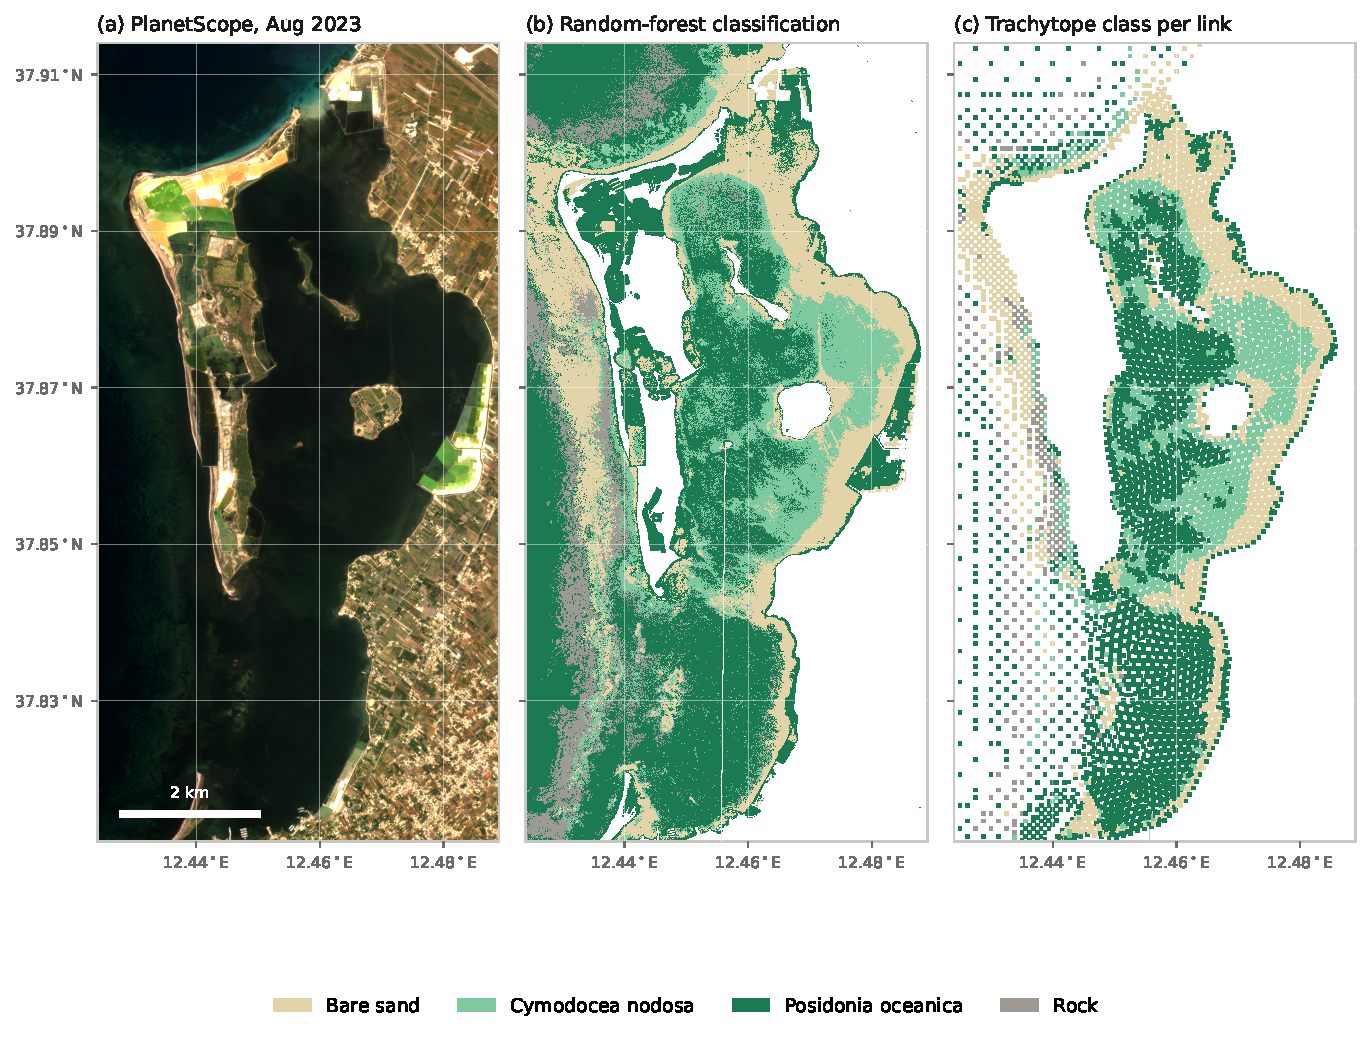
\includegraphics[width=\textwidth]{seagrass_classification}
  \caption{The seagrass map from imagery to model input. (a) PlanetScope
  SuperDove August 2023 median composite. (b) The random-forest classification,
  with the six output classes collapsed to the four seagrass classes.
  (c) The dominant class at each flow link, from the classification file
  the model reads, showing the mesh resolution the classification is sampled
  onto. The classification is computed over the whole scene, but only links
  inside the lagoon carry a canopy class.}
  \label{fig:seagrass}
\end{figure}

\subsection{Observational data and validation metrics}
\label{sec:methods_validation}

Water level was recorded at ten-minute resolution at three stations, BocaNord
at the northern inlet, BocaSud near the southern inlet, and AltaVilaEst on the
eastern flank of the central basin. Offshore performance was assessed at the
Marettimo tide gauge.

Water-level skill was quantified with the raw root-mean-square error, the
bias, and the anomaly root-mean-square error computed after removing the
respective means, together with the linear correlation and the ratio of
modelled to observed standard deviation. The three error measures are related
by $\mathrm{RMSE}^2 = \mathrm{bias}^2 + \mathrm{RMSE}_{\mathrm{anom}}^2$, so
reporting them jointly separates a constant reference-level offset from
genuine dynamic error in phase and amplitude. The first simulated day was
discarded as spin-up, over which the initial condition relaxes and the
transients it generates leave the basin.

Lagrangian skill was assessed against GPS-tracked surface drifters released in
the lagoon interior during the simulation window. Simulated trajectories were
obtained by advecting particles with OpenDrift \citep{Dagestad2018} through the
modelled surface current field, at an advection step of 300~s and with
positions written every 600~s. Scoring was restricted, for each drifter, to
the interval between its first and last observation, since the advection
continues to the end of the forcing while the deployments last between 0.4 and
7.2~h. A wind drift factor of 0.02 was applied to every member, since a sweep
over this parameter found no single value optimal across deployments and a
per-member value would have confounded the process attribution with a tuning
difference.

Agreement was quantified with the normalised cumulative
Lagrangian separation skill score of \citet{Liu2011}, which accumulates the
separation between modelled and observed positions and normalises it by the
distance travelled by the observed drifter, and with the endpoint proximity,
the separation between modelled and observed positions at the end of each
deployment. \citet{Revelard2021} discuss the sensitivity of this class of
metric to the normalisation choice in coastal applications.

\subsection{Numerical experiments}
\label{sec:methods_experiments}

Eight simulations were run over the same nine-day window, from the same initial
condition and with identical boundary and atmospheric forcing, so that the
differences between them isolate individual model components. All eight share
the mesh, and all wrote station output every 600~s and gridded output every
1800~s, so the comparison is not affected by differences in output sampling.

Members are identified by a three-slot code whose slots mark wave coupling,
seagrass canopy and mobile bed in that order, carrying \texttt{W}, \texttt{V}
or \texttt{M} where the factor is active and a dash where it is not. The eight
are \texttt{{-}{-}{-}}, \texttt{{-}V{-}}, \texttt{W{-}{-}}, \texttt{WV{-}},
\texttt{{-}{-}M}, \texttt{{-}VM}, \texttt{W{-}M} and \texttt{WVM}, and the code
is used throughout the results.

The design is a complete factorial in three factors, wave coupling, seagrass
canopy and bed mobility, and all eight cells were obtained. The process
attribution is made on the four fixed-bed members, a two-factor design in wave
coupling and canopy, and the four mobile-bed members form a sensitivity arm,
the critical shear stress for erosion not having been constrained against a
repeated bathymetric survey. Each vegetated member is a three-day segment
restarted on 7~July from the state of the bare member of the same cell, so the
two members of a pair share the first six days and differ by the canopy over
the window in which they are scored. In the mobile-bed members suspended
sediment does not contribute to the density field, and erodible sediment is
confined to depths above 15 to 20~m, where waves can plausibly move it
(Section~S5). The effect of the mobile bed on transport was traced with two
segments of the wave-coupled mobile-bed member without canopy, restarted on
7~July from its state on that date, one with the bed updated as in the member
and one with the bed held at that state.

The whole ensemble was also repeated from a vertically uniform column, at
24~$^\circ$C and 37.5 outside the lagoon and with the same hypersaline value
inside it. The horizontal and vertical resolution, a time-step limit by the
vertical fluxes, and the host and decomposition were tested on the uncoupled
fixed-bed configuration without canopy, as described in Section~S6.
